\begin{minipage}{10 cm}{
\Large
\textit{   Un niñito le dijo a su amigo: ``Mira yo le enseñé a mi perro Tobi a silbar''. El otro niño puso su oreja junto a la trompa del perro y dijo:``Yo no lo oigo silba''. El pequeño profesor respondió:``Yo dije que le enseñé, no dije que aprendió.''} \normalsize Anónimo...
}
\end{minipage}
\begin{minipage}{6 cm}{
\begin{center}
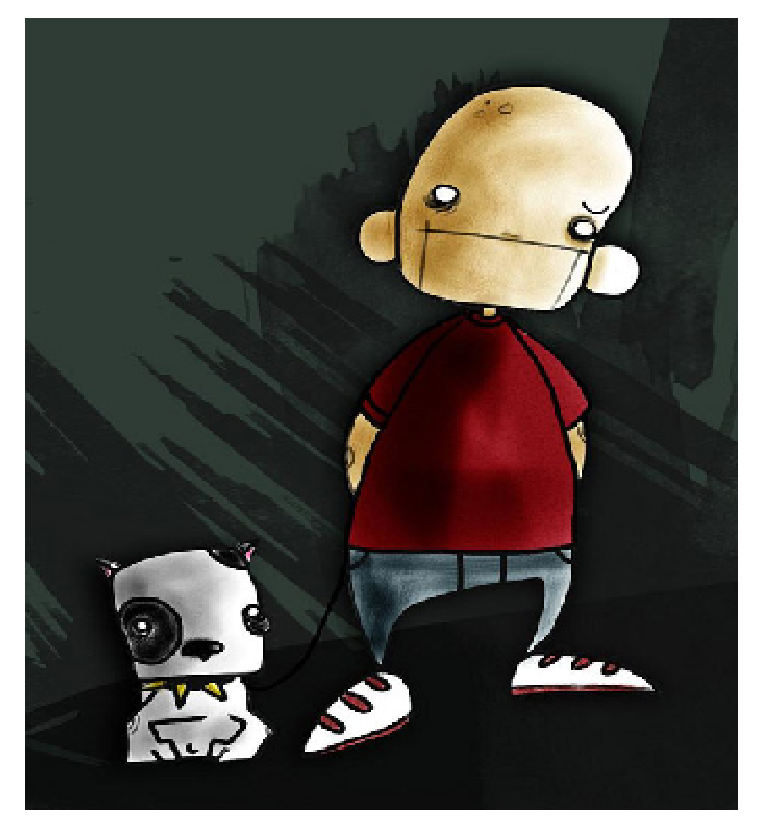
\includegraphics[scale=0.4]{a-fig1}
%\caption{Tobi y su perro}
\end{center}
}
\end{minipage}

\section*{¿Qué pasó con Tobi?}
\begin{itemize}
\item Es posible que el pequeño profesor no haya aplicado la metodología adecuada
\item Otra hipótesis es que Tobi no posea la capacidad para aprender a silbar
\item Una tercera hipótesis, es que a Tobi no le interesa aprender a silbar
\end{itemize}

\section*{Análisis de este caso}
\begin{itemize}
\item El interés y la necesidad de aprender algo, tienen que nacer de adentro
\item La función del profesor, es estimular que se genere esa necesidad y facilitar que esa necesidad pueda satisfacerse 
\end{itemize}

\section*{Conclusiones}
\begin{itemize}
\item Nadie puede aprender por otros, el interés por el aprendizaje debe generarse en el interior de la persona
\item Las materias no tiene una existencia real aunque estén escritas en los libros, lo que existe son las personas y sus problemas, por tanto es menos importante almacenar información y es mas importante el interés por aprender
\item Las personas aprenden lo que les interesa
\end{itemize}